

\subsection{Specifying the Plotted Range}

\begin{pgfplotsxykeylist}{\x min=\marg{coord},\x max=\marg{coord},min=\marg{coord},max=\marg{coord}}
These options allow to define the axis limits, i.e.\ the lower left and the upper right corner. Everything outside of the axis limits will be clipped away.

Each of these keys is optional, and missing limits will be determined automatically from input data. Here, the |min| and |max| keys set limits for $x$, $y$ and $z$ to the same \meta{coord}.

If $x$-limits have been specified explicitly and $y$-limits are computed automatically, the automatic computation of $y$-limits will only considers points which fall into the specified $x$-range (and vice--versa). The same holds true if, for example, only |xmin| has been provided explicitly: in that case, |xmax| will be updated only for points for which $x \ge \,$|xmin| holds. This feature can be disabled using |clip limits=false|. 

Axis limits can be increased automatically using the |enlargelimits| option.
\begin{codeexample}[]
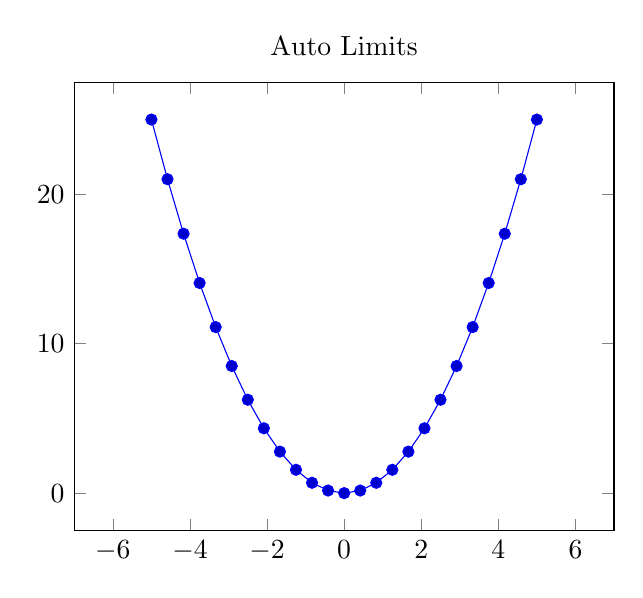
\begin{tikzpicture}
	\begin{axis}[title=Auto Limits]
	\addplot {x^2};
	\end{axis}
\end{tikzpicture}
\end{codeexample}

\begin{codeexample}[]
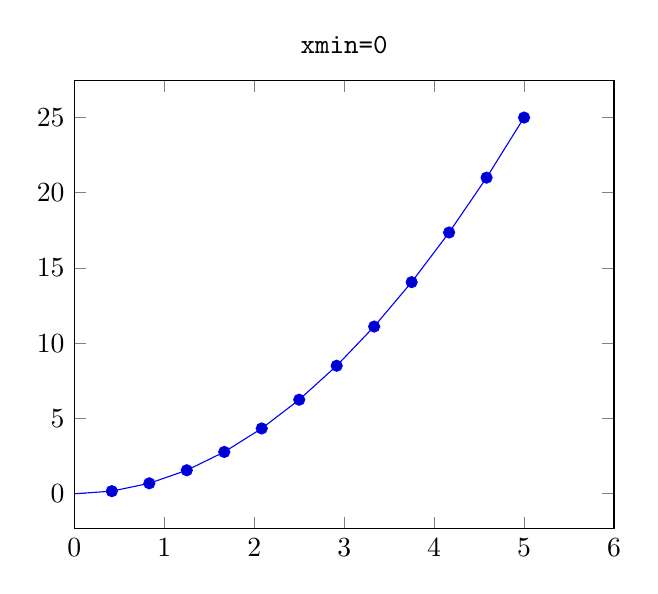
\begin{tikzpicture}
	\begin{axis}[title={\texttt{xmin=0}},xmin=0]
	\addplot {x^2};
	\end{axis}
\end{tikzpicture}
\end{codeexample}

\begin{codeexample}[]
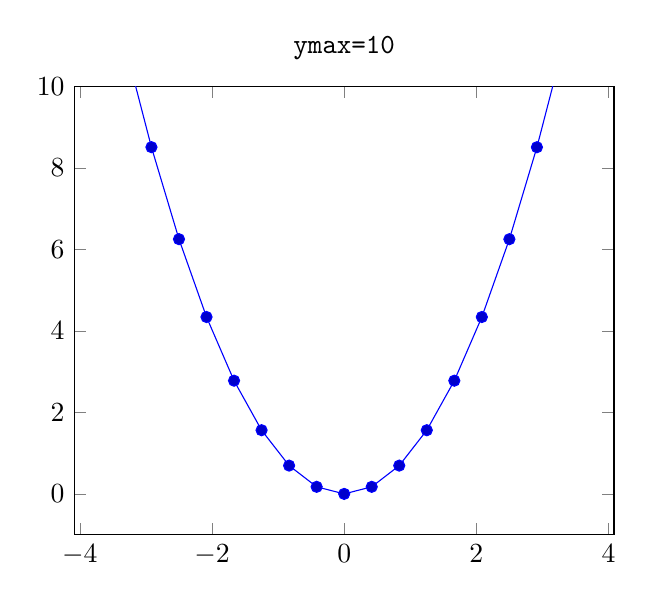
\begin{tikzpicture}
	\begin{axis}[title={\texttt{ymax=10}},ymax=10]
	\addplot {x^2};
	\end{axis}
\end{tikzpicture}
\end{codeexample}

	Note that even if you provide |ymax=10|, data points with $y>10$ will still be visualized -- producing a line which leaves the plotted range.

	See also the |restrict x to domain| and |restrict x to domain*| keys -- they allow to discard or clip input coordinates which are outside of some domain, respectively.


	During the visualization phase, i.e.\ during |\end{axis}|, these keys will be set to the final axis limits. You can access the values by means of |\pgfkeysvalueof{/pgfplots/xmin}|, for example:
\begin{codeexample}[]
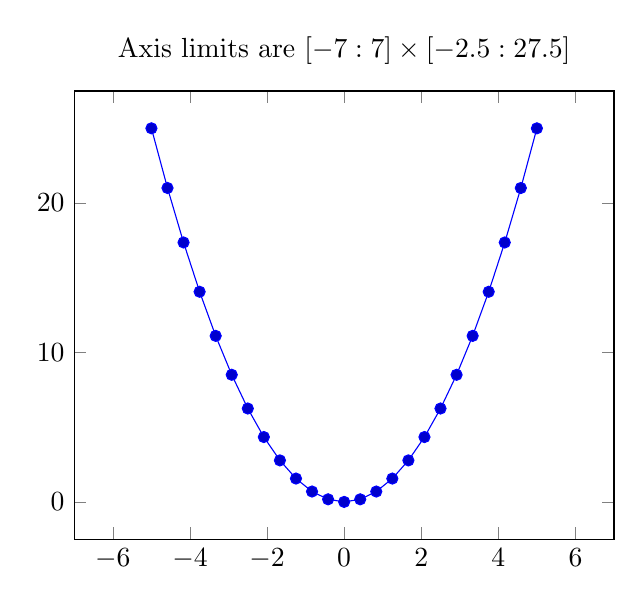
\begin{tikzpicture}
\begin{axis}[
 % Show (automatically) computed limits:
 title={
  Axis limits are 
  $
 [\pgfmathprintnumber{\pgfkeysvalueof{/pgfplots/xmin}}
 :\pgfmathprintnumber{\pgfkeysvalueof{/pgfplots/xmax}}
 ]  \times 
 [\pgfmathprintnumber{\pgfkeysvalueof{/pgfplots/ymin}}
 :\pgfmathprintnumber{\pgfkeysvalueof{/pgfplots/ymax}}
 ]$ },
]
	\addplot {x^2};
\end{axis}
\end{tikzpicture}
\end{codeexample}
	\label{page:access:limits}
	This access is possible inside of any axis description (like |xlabel|, |title|, |legend entries| etc.) or any annotation (i.e. inside of |\node|, |\draw| or |\path| and coordinates in |(axis cs:|\meta{x}|,|\meta{y}|)|), but not inside of |\addplot| (limits may not be complete at this stage).
\end{pgfplotsxykeylist}

\begin{pgfplotsxykey}{\x mode=\mchoice{normal,linear,log} (initially normal)}
	Allows to choose between linear (=normal) or logarithmic axis scaling or logplots for each $x,y,z$-combination.

	Logarithmic plots use the current setting of |log basis x| and its variants to determine the basis (default is $e$).
	% FIXME : replicated in pgfplots.reference.scaling.tex
\end{pgfplotsxykey}

\begin{pgfplotsxykey}{\x\ dir=\mchoice{normal,reverse} (initially normal)}
\pgfkeys{/pdflinks/search key prefixes in/.add={/pgfplots/,}{}}
	Allows to reverse axis directions such that values are given in decreasing order.
\label{key:pgfplots:xydir}
\begin{codeexample}[]
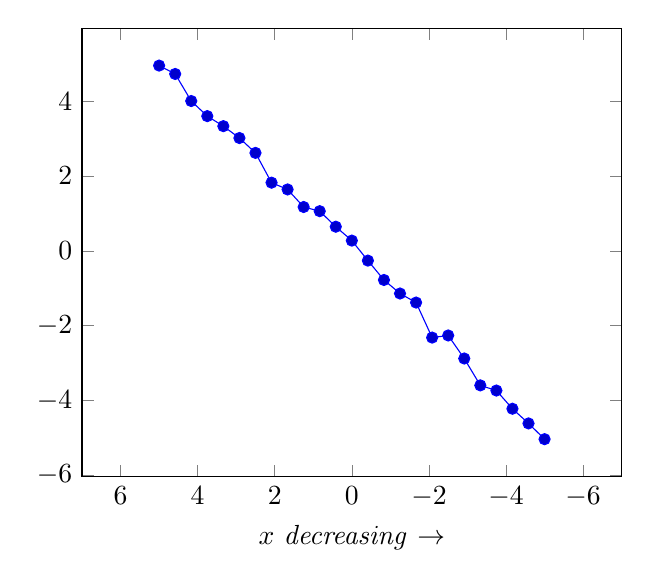
\begin{tikzpicture}
\begin{axis}[
	xlabel=$x$ \emph{decreasing} $\to$,
	x dir=reverse]
	\addplot {x+rand*0.3};
\end{axis}
\end{tikzpicture}
\end{codeexample}

\begin{codeexample}[]
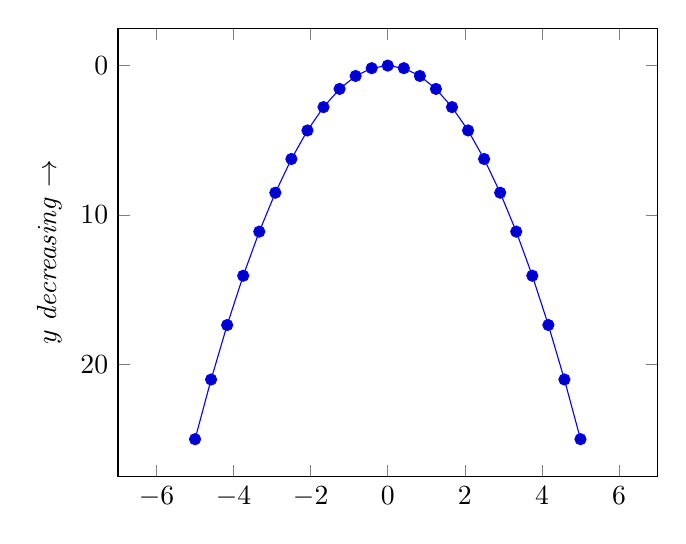
\begin{tikzpicture}
\begin{axis}[
	ylabel=$y$ \emph{decreasing} $\to$,
	y dir=reverse]
	\addplot {x^2};
\end{axis}
\end{tikzpicture}
\end{codeexample}

	Note that axis descriptions and relative positioning macros will stay at the same place as they would for non--reversed axes.
\begin{codeexample}[]
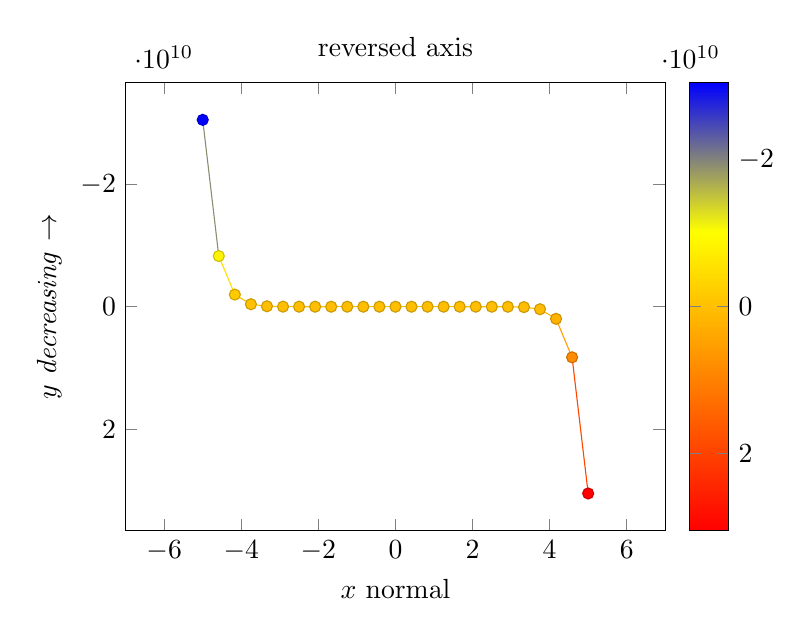
\begin{tikzpicture}
\begin{axis}[
	ylabel=$y$ \emph{decreasing} $\to$,
	xlabel=$x$ normal,
	title=reversed axis,
	y dir=reverse,
	colorbar,
	colorbar style={y dir=reverse}]
	\addplot+[mesh,scatter] {x^15};
\end{axis}
\end{tikzpicture}
\end{codeexample}

	Note that |colorbar|s won't be reversed automatically, you will have to reverse the sequence of color bars manually in case this is required as in the preceding example.
\end{pgfplotsxykey}

\begin{pgfplotskey}{clip limits=\mchoice{true,false} (initially true)}
	Configures what to do if some, but not all axis limits have been specified explicitly. In case |clip limits=true|, the automatic limit computation will \emph{only} consider points which do not contradict the explicitly set limits. 

	This option has nothing to do with path clipping, it only affects how the axis limits are computed.
\end{pgfplotskey}

\begin{pgfplotsxykeylist}{%
	enlarge \x\ limits=\mchoice{auto,true,false,upper,lower,\meta{val},value=\meta{val},abs value=\meta{val},\\ abs=\meta{val},rel=\meta{val}} (initially auto),
	enlargelimits=\meta{common value}}
Enlarges the axis size for one axis (or all of them for |enlargelimits|) somewhat if enabled.

You can set |xmin|, |xmax| and |ymin|, |ymax| to the minimum/maximum values of your data and |enlarge x limits| will enlarge the canvas such that the axis doesn't touch the plots.

	 The value \declaretext{true} enlarges the lower and upper limit.

	 The value \declaretext{false} uses tight axis limits as specified by the user (or read from input coordinates).

	 The value \declaretext{auto} will enlarge limits only for axis for which axis limits have been determined automatically.
	For three--dimensional figures, the \declaretext{auto} mechanism applies only for the $z$ axis. The $x$ and $y$ axis won't be enlarged. 
\begin{codeexample}[]
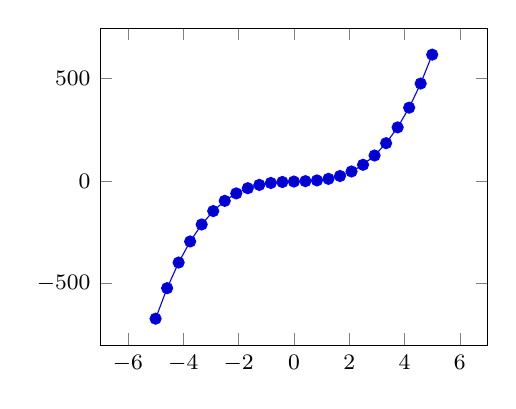
\begin{tikzpicture}
	\begin{axis}[small]
		\addplot {5 * x^3 - x^2 + 4*x -2};
	\end{axis}
\end{tikzpicture}
\end{codeexample}


	 Specifying a number \declaretext{val}ue like `|enlarge x limits=0.2|' will enlarge lower and upper axis limit relatively. The following example adds $20\%$ of the axis limits on both sides:
\begin{codeexample}[]
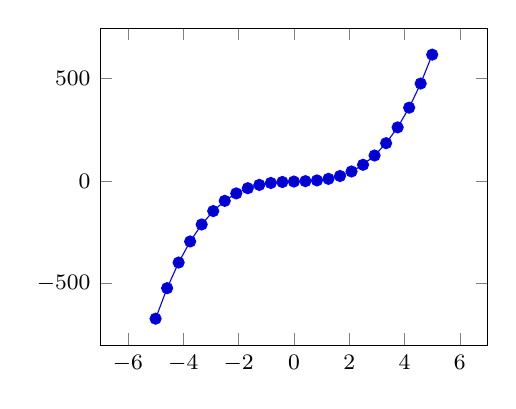
\begin{tikzpicture}
	\begin{axis}[small,enlarge x limits=0.2]
		\addplot {5 * x^3 - x^2 + 4*x -2};
	\end{axis}
\end{tikzpicture}
\end{codeexample}
	\noindent The choice \declaretext{rel=}\marg{value} is the same as |true,value=|\marg{value}, i.e.\ it activates relative enlargement for both |upper| and |lower| limit.

	 The value \declaretext{upper} enlarges only the upper axis limit while \declaretext{lower} enlarges only the lower axis limit. In this case, the amount added to the respective limit can be specified using the \declaretext{value=}\marg{val} key. It can be combined with any of the other possible values. For example, 

		|\pgfplotsset{enlarge x limits={value=0.2,upper}}|
	
	will enlarge (only) the upper axis limit by $20\%$ of the axis range. Another example is

		|\pgfplotsset{enlarge x limits={value=0.2,auto}}|

	which changes the default threshold of the \declaretext{auto} value to $20\%$.
\begin{codeexample}[]
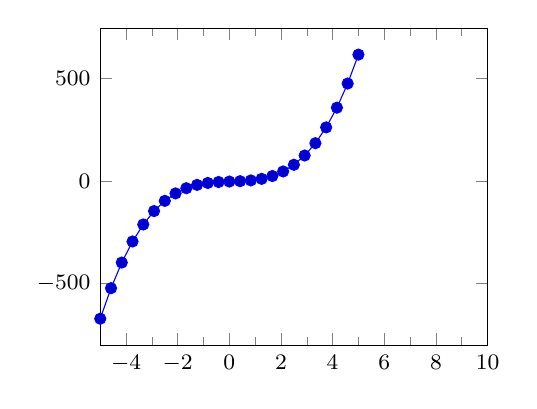
\begin{tikzpicture}
	\begin{axis}[small,minor x tick num=1,
		enlarge x limits={rel=0.5,upper}
	]
		\addplot {5 * x^3 - x^2 + 4*x -2};
	\end{axis}
\end{tikzpicture}
\end{codeexample}


	 While |value| uses relative thresholds, \declaretext{abs value} accepts absolute values: it adds an absolute value to the selected axis. The choice \declaretext{abs=}\marg{value} is the same as |true,abs value=|\marg{value}, i.e.\ it adds an absolute value to both |upper| and |lower| limit:
\begin{codeexample}[]
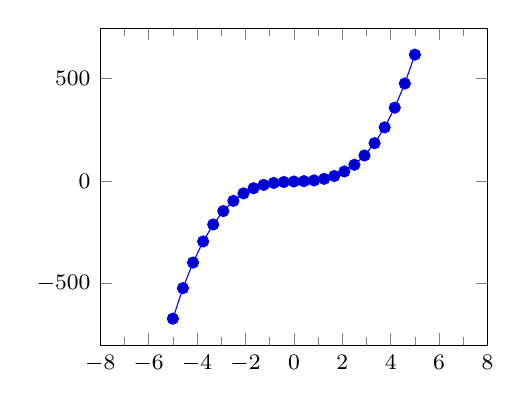
\begin{tikzpicture}
	\begin{axis}[small,minor x tick num=1,
		enlarge x limits={abs=3}
	]
		\addplot {5 * x^3 - x^2 + 4*x -2};
	\end{axis}
\end{tikzpicture}
\end{codeexample}
	\noindent Here, we enlarged by $3$ units of the $x$ axis. Note that you can also specify \emph{dimensions} like |1cm|:
\begin{codeexample}[]
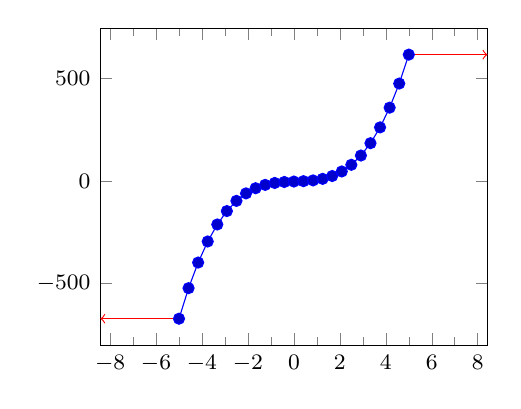
\begin{tikzpicture}
	\begin{axis}[small,minor x tick num=1,
		enlarge x limits={abs=1cm}
	]
		\addplot {5 * x^3 - x^2 + 4*x -2}
		  coordinate[pos=0] (first)
		  coordinate[pos=1] (last);

		\draw[red,->] (first) -- ++(-1cm,0pt);
		\draw[red,->] (last) --  ++(1cm,0pt);
	\end{axis}
\end{tikzpicture}
\end{codeexample}
	\noindent Technically, the use of absolute dimensions is a little bit different. For example, it allows to enlarge by more than |width| which is impossible for all other choices. \PGFPlots\ will try to fulfill both the provided |width|/|height| and the absolute axis enlargements. If it fails to do so, it will give up on |width|/|height| constraints and print a warning message to your log file. See also the key |enlargelimits respects figure size|.\index{Errors!enlargelimits respects figure size=true: could not respect the prescribed width/height}

	\paragraph{Attention:} |abs value| is applied \emph{multiplicatively} for logarithmic axes! That means |abs value=10| for a logarithmic axis adds $\log 10$ to upper and/or lower axis limits.
\begin{codeexample}[]
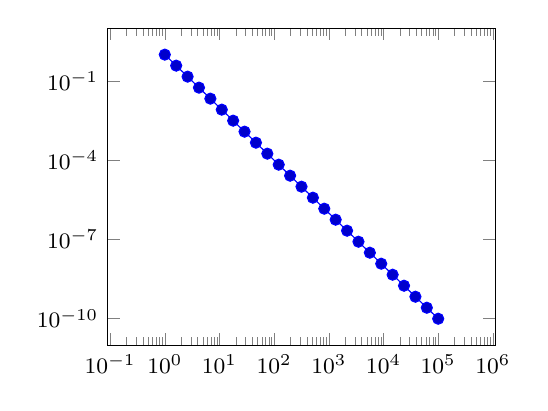
\begin{tikzpicture}
	\begin{loglogaxis}[small,enlarge x limits={abs=11}]
		\addplot+[domain=1:100000] {x^-2};
	\end{loglogaxis}
\end{tikzpicture}
\end{codeexample}


	Note that |enlargelimits| is applied before any changes to axis limits are considered as part of |scale mode|: |enlargelimits| will always be applied. Afterwards, the choice |scale mode=scale uniformly| will enlarge limits once more in order to satisfy all scaling constraints. The two limit enlargements are independent of each other, i.e.\ even if you say |enlargelimits=false|, |scale mode| will still increase axis limits if this seems to be necessary. An exception for this rule is enlarge-by-dimension, i.e.\ something like |abs=1cm| (see |enlargelimits respects figure size| for this case).
	See |scale mode| (especially |scale mode=units only|) and |unit rescale keep size| for detail on how to disable limit enlargement caused by |scale mode|. 
\end{pgfplotsxykeylist}

\begin{pgfplotskey}{enlargelimits respects figure size=\mchoice{true,false} (initially true)}
	A key which is \emph{only} used for something like |enlarge x limits={abs=1cm}|, i.e.\ for enlarge-by-dimension. It controls if \PGFPlots\ will try to respect |width|/|height|. You should probably always leave it as its default unless you run into problems.

	If \PGFPlots\ fails to respect the figure size, it will print a warning message of sorts ``enlargelimits respects figure size=true: could not respect the prescribed width/height'' to your log file\index{Errors!enlargelimits respects figure size=true: could not respect the prescribed width/height}. 
	
\end{pgfplotskey}

\begin{pgfplotsxykeylist}{%
	log origin \x=\mchoice{0,infty} (initially infty),%
	log origin=\mchoice{0,infty} (initially infty)}%
	Allows to choose which coordinate is the logical ``origin'' of a logarithmic plot (either for a particular axis or for all of them).

	The choice |log origin=infty| is probably useful for stacked plots: it defines the ``origin'' in log--coordinates to be $-\infty$. To be compatibly with older versions, this is the default.

	The choice |log origin=0| defines the logarithmic origin to be the natural choice $\log(1)=0$. This is particularly useful for |ycomb| plots.
\end{pgfplotsxykeylist}

\begin{pgfplotskey}{update limits=\mchoice{true,false} (initially true)}
	Can be used to interrupt updates of the data limits (for example, for single |\addplot| commands).

	This has the same effect as |\pgfplotsinterruptdatabb| ... |\endpgfplotsinterruptdatabb|.
\end{pgfplotskey}

\begin{environment}{{pgfplotsinterruptdatabb}}
\index{Bounding Box Control!Disable \protect\emph{data} bounding box modifications}
	Everything in \meta{environment contents} will not contribute to the data bounding box.

	The same effect can be achieved with |update limits=false| inside curly braces.
\end{environment}
